
\chapter{Content Delivery} \label{chap:cn}{

The content delivery problem can be defined as the problem of efficiently distributing a file from an origin, possibly the creator, to a set of user. This problem arises every time a user tries to view a website, requests the delivery of an HTML file, watches a video on YouTube, requests the delivery of a video file and updates the Operating System (OS) of her computer, or requests a new ISO version of the OS. To address this problem, multiple approaches with different performance guarantees are employed. In this section, the most common content distribution methods will be discussed and compared.

\section{Client Server Model}{

The first approach to address content delivery is the client-server model. The client-server model relies on the existence of one or multiple servers operated by the file distributor \cite{Berson:245910}. Clients that want the file make a request to download it from the server and then the server responds back with the file. This paradigm is widely used to deliver the front-end of a website to the user. When a user visits a website such as google.com, the browser requests the HTML file from a Google server. This approach works perfectly for small HTML files. Companies can use cloud-services to vertically and horizontally scale their infrastructure to handle an increasing number of requests. However, as the file sizes and the number of requests increase, the scaling required eventually becomes prohibitively expensive. As a result, the website becomes slow and ultimately unavailable. The other disadvantage of this approach is that it relies on a single entity to distribute the file. If this entity becomes unavailable, chooses to censor a file or the government bans the access to the distributor then the file becomes unavailable.
}
\section{End-host Multicast}{

End-host multicast is an improvement over the client-server model that focuses on improving its performance in distributing larger files to multiple peers. There exist two versions of multicast. IP multicast relies on the idea that routers forward packets to multiple addresses. End-host multicast relies on the idea that each end-host sends the downloaded files to others when it finish downloading. Unfortunately, IP multicast, although technologically viable, is not widely supported by Internet-Service-Providers and as a result, it is a viable solution only for distributing content within a private network (e.g. a data center). End-host multicast relies on the idea that when nodes successfully finish downloading a file, they themselves distribute the file to two other nodes. The benefit of this approach is that it moves some of the load from the distribution server to end-hosts. Various protocols such as Overcast \cite{jannotti2000overcast} and ALMI \cite{verma2001almi} have been designed in the past decades. All the designed protocols create a single tree structure as illustrate in Figure \ref{fig:ipMulti} to distribute the file.

\begin{figure}[htb!]
\centering
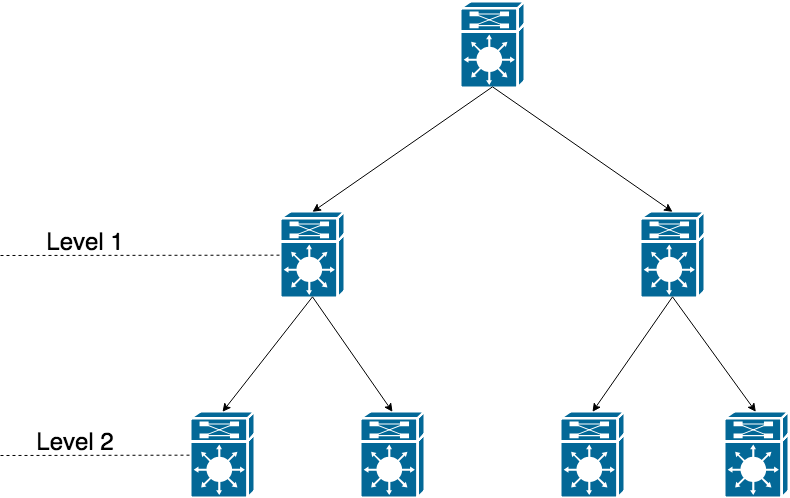
\includegraphics[width=0.95\textwidth]{./pics/Ip-multi.png}
\caption{End-host multicast single tree structure and propagation of data}
\label{fig:ipMulti}
\end{figure}

The main issue with the single tree structure is poor load balancing among nodes. The first observation is that nodes in the lowest level do not contribute at all to the distribution of the file. Additionally, if a node at a high level, close to level 0, fails to distribute the file or is terribly slow, then the whole subtree that depends on it will not receive the file.

}
\section{BitTorrent}{

BitTorrent is a peer-to-peer (P2P) file distribution protocol that was designed by Brah Cohen in 2001 \cite{BramCohen2008BitTorrentSpecification}. BitTorrent was a more decentralized version of previous systems such as Napster and Kazaa. According to the BitTorrent protocol nodes that are interested in downloading the same file are organized in swarms. Within the swarm, nodes request chunks of the file from their neighbors.

A really innovative idea in the design of the BitTorrent protocol is the "tit-for-tat" mechanism. This mechanism incentivizes nodes to contribute to the distribution of the files because otherwise they will be choked by their neighbors. This means that in order to download all the chunks of the file, one must also upload chunks of they file you already have.

To distribute a file using the BitTorrent protocol, the creator must create a torrent file that specifies the address of the swarm-tracker, the chunks that compose the file and their hash. The torrent file is uploaded in a torrent repository and then users can download the torrent file and feed it to a BitTorrent client. Finally, the BitTorrent client will download the original file. In terms of performance and robustness, BitTorrent has already proved itself  \cite{BitPerf}. According to the study in \cite{6912519}, P2P content distribution constitutes 16\% of the download traffic of two major European ISPs. Furthermore, companies like Facebook, Twitter, Blizzard \footnote{\url{http://us.blizzard.com/es-mx/company/about/legal-faq.html}, Access Date: 7 Aug. 2018}, and Linux foundation \footnote{\url{https://linuxtracker.org/}, Access Date: 7 Aug. 2018} use their in-house implementation of the BitTorrent protocol to distribute data among data centers or to their users.

The main robustness drawback of the BitTorrent protocol is that it has single-point of failure. If the swarm-tracker becomes unavailable (due to censorship), then users have no mean to enter the swarm and download the file. In terms of performance, the main issue with BitTorrent is data duplication. This means that if the same file is uploaded with a different name, then there will be two torrent swarms that do not communicate with one another.
}
\section{IPFS}{
IPFS\footnote{Interplanetary File System} is also a peer-to-peer (P2P) file distribution protocol that was designed by the Protocol Labs company and 
Juan Benet in 2014 \cite{benet2014ipfs}. Protocol Labs received 257M in funding in 2017, that was the biggest Initial Coin Offering (ICO) at the time \footnote{\url{https://coinlist.co/filecoin}, Access Date: 7 Aug. 2018}. IPFS is a decentralized file distribution protocol that shares many ideas with BitTorrent but uses the hash of the file as its address in the network. IPFS can be thought of as a single swarm BitTorrent network. Similarly to BitTorrent, IPFS uses the "tit-for-tat" mechanism to incentivize users to distribute their files. However, as users are organized in a single swarm, a user can distribute chunks of a different file than the ones she tries to download.

Users entering the IPFS network download a ledger that contains a list of nodes that participate in the network. Then the node can make a connection to the users she sees in the ledger. Upon establishing a connection to the network, the user can locate other nodes that have the files she wants and download the files from them. In return, she uploads the files she already has. This is implemented with two lists. Each user publishes to the network her want list, i.e. list of file chunks that she wants, and the have list, i.e. a list of file chucks that she has.

As an optimization to avoid storing duplicate data in the network, files are stored based on their hash, thus constructing a Merkle Tree \cite{MerkleTrees} with different files and versions of files. Each file is identified with an IPFS link that has the following form:
\begin{center}
/ipfs/\textit{file\_hash}/
\end{center}
IPFS links are resolved using the IntePlanetary-Name-System (IPNS) which is similar to Domain-Name-System (DNS) but for IPFS links. As an example, a website could be hosted on IPFS using the following link:

\begin{center}
localhost:8080/ipfs/\textit{hash(my\_website.html)} 
\end{center}


The main disadvantage of IPFS at the time of writing is the exponential increase of available files. Take for example the HTML page for the landing page of a website. Small differences in HTML would result in a completely different hash. As a result, IPNS that resolves the name of the website to an IPFS address must constantly be updated, even for small changes of files. Another performance issue arises from the immaturity of the project. As the project is in an early Alpha development stage many operations are not optimized. As we will later demonstrate, this suboptimal operations severely limit its practical performance.
}

\section{Summary}{

A comparison between the content distribution protocols discussed in this section is presented in Table \ref{tab:CNComp}. The comparison focuses on the scalability of the protocols as the number of nodes increases, the existence of failure points within the network and how balanced the load is among the participants in the network.

\begin {table}[htb!]
\caption {Comparison of content distribution protocols} \label{tab:CNComp} 
\begin{center}
 \begin{tabular}{|c| c|c| c|c| c|c| c|} 
 \hline
  Protocol & Scalability & Point of failure & Load Balance \\ [0.5ex] 
 \hline
 Client-server & Depends on server & Server & Poor  \\ 
 \hline
 End-host multicast  & Depends on each node & Multiple partial & Poor \\
 \hline
 BitTorrent  & No scalability issues & Tracker server & Evenly Distributed \\
 \hline
 IPFS  & No scalability issues & None & Evenly Distributed \\
 \hline
\end{tabular}
\end{center}
\end {table}

}

}